\section{Additional Diagnostics}\label{app:diagnostics}

\subsection{Graph Density Statistics}

Table~\ref{tab:density_stats} compares graph densities across methods.

\subsection{DAGMA Threshold Sensitivity}

Figure~\ref{fig:threshold} reports the sensitivity of Los-loop results to the DAGMA threshold $\tau$ (equivalently, to the learned graph's sparsity). RMSE decreases monotonically as sparser graphs are selected, and T-GCN-MultiGSL-Mix attains its best RMSE near the operating point of 30 edges used throughout the main text.

\begin{figure}[ht]
\centering
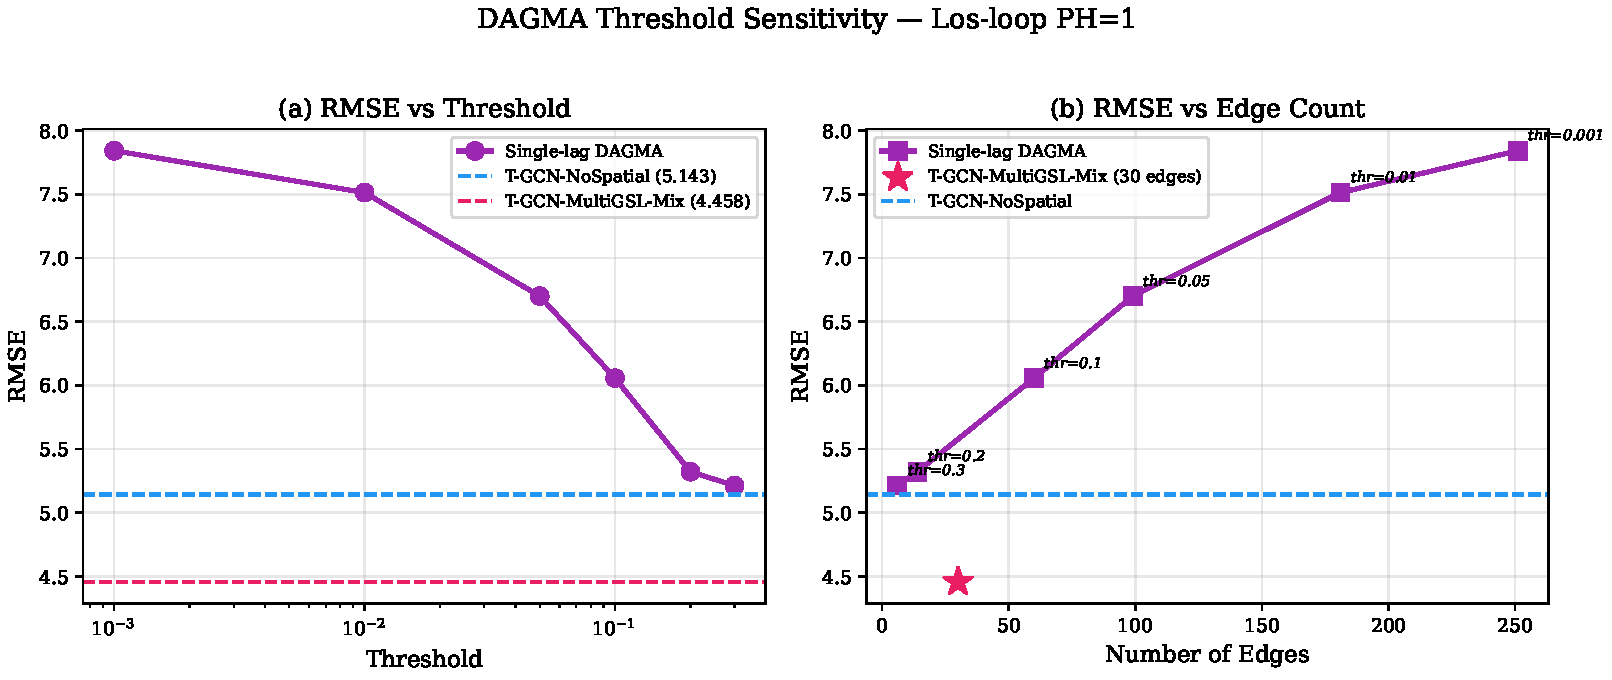
\includegraphics[width=0.9\textwidth]{figures/fig6_threshold_sensitivity.pdf}
\caption{DAGMA threshold sensitivity (Los-loop, PH=1, seed=42). (a) RMSE decreases monotonically with higher thresholds. (b) RMSE vs.\ edge count: T-GCN-MultiGSL-Mix (star) achieves the best performance with 30 edges.}
\label{fig:threshold}
\end{figure}

\subsection{Training Convergence (Revision Experiments)}

Figure~\ref{fig:convergence_rev} shows the training loss curves for the three main methods on Los-loop and SZ-Taxi. All methods converge within 50 epochs, with T-GCN-MultiGSL-Mix achieving the lowest final training loss on Los-loop; on SZ-Taxi the curves are close, consistent with the marginal performance difference.

\begin{figure}[ht]
\centering
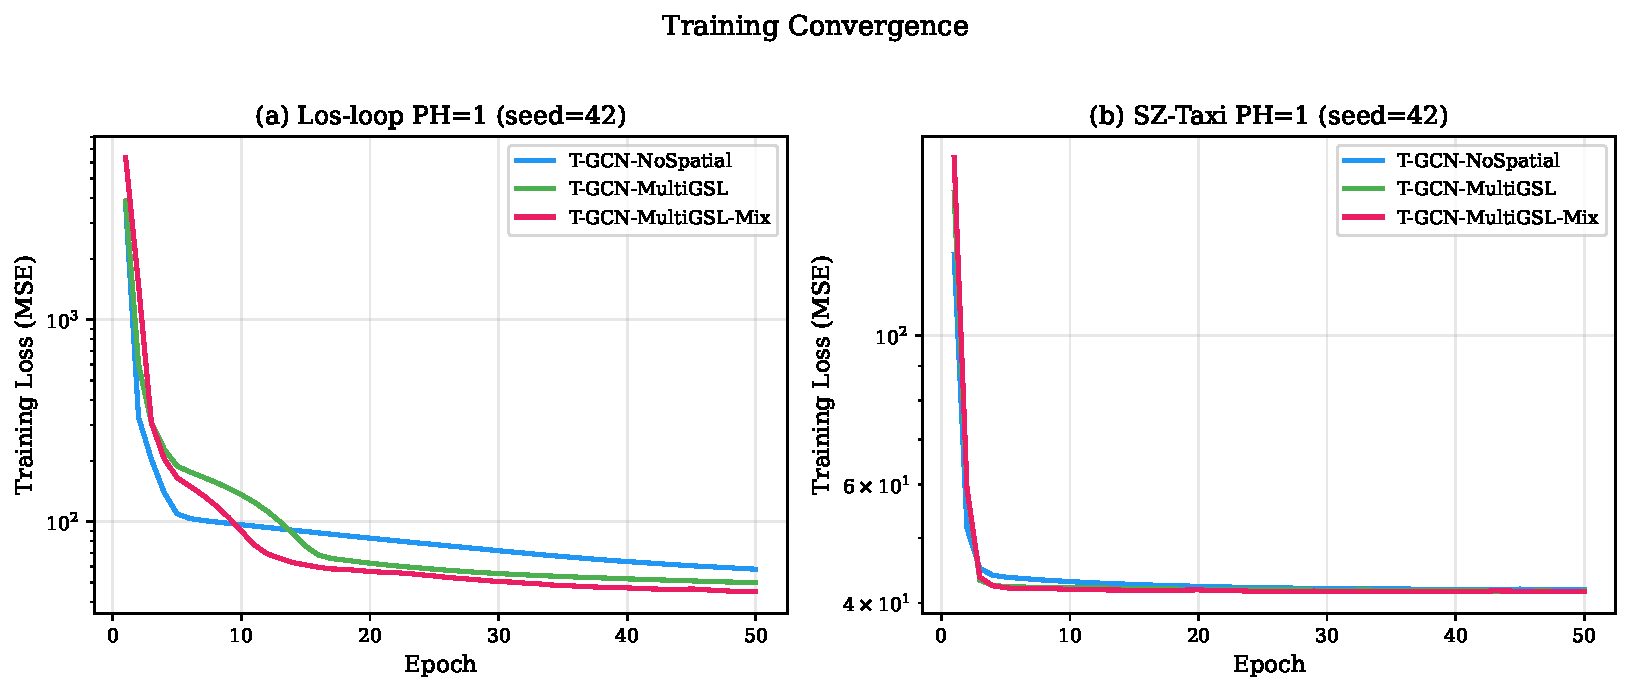
\includegraphics[width=0.9\textwidth]{figures/fig8_convergence.pdf}
\caption{Training convergence (PH=1, seed=42). (a) Los-loop: T-GCN-MultiGSL-Mix converges to the lowest training loss. (b) SZ-Taxi: all methods show similar convergence, consistent with the marginal performance difference.}
\label{fig:convergence_rev}
\end{figure}

\subsection{Parameter-Matched Control}

Figure~\ref{fig:param_control_app} visualizes the parameter-matched control of the main text (Table~\ref{tab:param_control}).

\begin{figure}[ht]
\centering
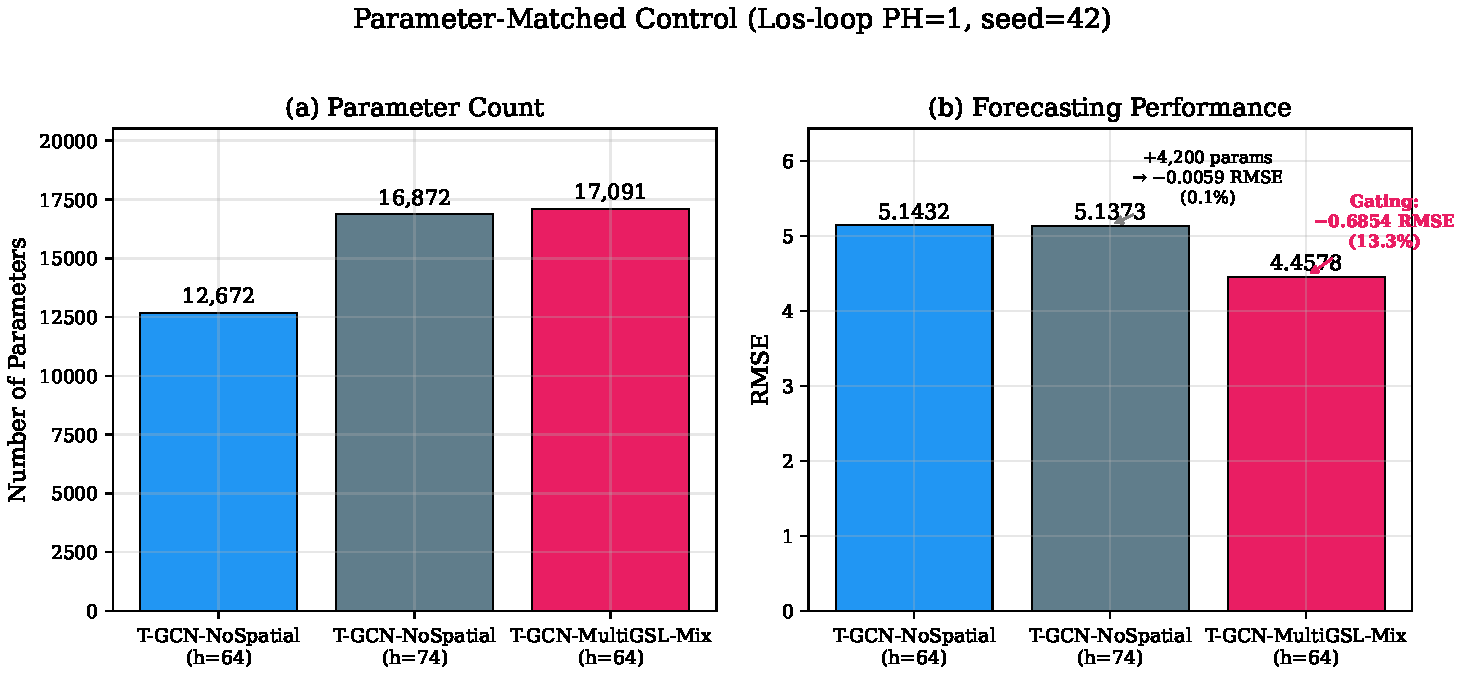
\includegraphics[width=0.9\textwidth]{figures/fig4_param_control.pdf}
\caption{Parameter-matched control (Los-loop, PH=1, seed=42). (a) Parameter counts are comparable. (b) Adding 35\% more parameters to T-GCN-NoSpatial improves RMSE by only 0.1\%, while the gating architecture provides 13.3\% improvement.}
\label{fig:param_control_app}
\end{figure}

\begin{table}[ht]
\centering
\caption{Graph density comparison (Los-loop, $N=207$).}
\label{tab:density_stats}
\begin{tabular}{lcc}
\toprule
\textbf{Graph} & \textbf{Edges} & \textbf{Density} \\
\midrule
Physical & 2833 & 0.0660 \\
T-GCN-NoSpatial (identity) & 207 & 0.0048 \\
T-GCN-MultiGSL ($\tau$=0.1) & 30 & 0.0007 \\
T-GCN-MultiGSL-Mix ($\tau$=0.1) & 30 & 0.0007 \\
\bottomrule
\end{tabular}
\end{table}

\subsection{DAGMA Computational Cost}

Multi-lag DAGMA runtime on standard hardware (RTX 3090):
\begin{itemize}
    \item SZ-Taxi ($624 \times 624$): approximately 100 minutes per prediction horizon
    \item Los-loop ($828 \times 828$): approximately 240 minutes per prediction horizon
\end{itemize}
Total computation for the 8 primary DAGMA runs (2 datasets $\times$ 4 PHs): approximately 24 hours; the additional 15-minute-resolution DAGMA run (Section~\ref{sec:los15min}) took approximately 4 hours.

For reference, the contemporaneous single-graph fits of Section~\ref{sec:gsl_baseline} (207 variables, $\lambda_1 = 0.02$, warm-up 30{,}000 / max 60{,}000 iterations) took approximately 15--17 minutes per horizon on 4 CPU cores, and archived 156-variable SZ-Taxi audit fits took approximately 52--76 minutes each. A sliding-window time-varying extension would multiply these per-fit costs by the number of windows.
